\subsection{Xarxa d'interconnexió}

Entenent que tenim un nombre relativament reduït d'unitats i que volem dedicar tantes unitats com 
sigui possible a nodes de còmput, volem reduir el nombre d'unitats que dediquem als commutadors. Per aconseguir aquesta fita, necessitem que cada commutador tingui el màxim
nombre de ports per unitat.
Com efecte col·lateral d'aquesta estratègia ens veiem amb un sistema que pràcticament es veu forçat a utilitzar una topologia de xarxa de tipus malla.

Pel que fa a distribuïdors, ens vam centrar en \textit{Mallanox Technologies}. A la pàgina web
\cite{mellanox-web} de la companyia, vam trobar commutadors \textit{InfiniBand} de diferents preus
i velocitats (com més ports major és la velocitat). A la taula \ref{tab:intercon} hem recollit els 
diferents models candidats a ser utilitzats en el nostre sistema.

\begin{table}[H]
\begin{adjustwidth}{-.5in}{-.5in}  
    \begin{center}
        \centering
        \scalebox{1.0}{
        \begin{centering}
            \begin{tabular}{l||c|c|c}
                \hline
                \cellcolor[HTML]{FFFFFF}Model         & Ports & Speed (Gb/s) & Preu (\$) \\ \hline \hline \rowcolor[HTML]{EFEFEF}
                MSX6012F-2BFS \cite{mellanox_msx6012f-2bfs} & 12      & 56           &  9309.00  \\ 
                MSX6018F-1SFS \cite{mellanox_msx6018f-1sfs} & 18      & 56           & 14791.00  \\ \rowcolor[HTML]{EFEFEF} 
                MSB7800-ES2F \cite{mellanox_msb7800-es2f}  & 36      & 100          & 25633.00  \\ 
                MQM8700-HS2F \cite{mellanox_mqm8700-hs2f}  & 40      & 200          & 29629.00  \\ \hline
            \end{tabular}
        \end{centering}
        }
    \caption{Comparació entre les diferents configuracions dels nodes.}
    \label{tab:intercon}
    \end{center}
\end{adjustwidth}
\end{table}

La quantitat de commutadors que utilitzem en el nostre sistema és un factor clau que marca,
tan el preu, com el rendiment, d'aquest. D'altre banda, però, afecta diferent als dos paràmetres,
anteriors en funció dels altres components. Per tan no podem determinar encara quina serà la
millor configuració. No obstant, si que podem reduir el rang de configuracions, per tal que
l'anàlisi sigui més amè.

Ja que utilitzem una topologia de tipus malla completa, el nombre de connexions $C$ a nodes de còmput
que podrà tenir la xarxa ve marcat per el nombre de ports $P$ del que disposa cada commutador, així
com el nombre de commutadors $N$ que tingui el sistema. Deduïm que el nombre de connexions
que podrà haver al sistema ve determinat per $C = N \times ( P - N + 1 ) = -N^2 + N(P+1)$.
A la figura \ref{fig:connections} podem veure quin és el comportament d'aquesta funció quan incrementem
el nombre de commutadors, aquesta figura consta del comportament dels commutadors, així com del nombre 
d'unitats que queden disponibles. Pel nostre sistema estudiarem aquelles configuracions que s'acostin 
més a la línia de punts. Cal entendre que si són més avall de la línia de punts vol dir que estem perden connexions
i que possiblement ens quedi espai lliure a l'armari. D'altra banda, si som més amunt de la línia 
significa que ja tenim les connexions necessàries per omplir els dos armaris; incrementar el nombre de connexions
només ens portaria a desaprofitar-les (assumim que mínim una U per node).

Llavors, a partir d'aquest argument podem desglossar les diferents configuracions que val la pena explorar:
\begin{itemize}
  \item El cas del model \textit{MSX6012F-2BFS} no l'analitzarem, ja que no hi ha cap configuració òptima per la topologia utilitzada.
  \item Pel cas del model \textit{MSX6018F-1SFS}, tenint en compte que tenim divuit ports, analitzarem les configuracions amb sis i set commutadors.
  \item Pel cas del model \textit{MSB7800-ES2F}, amb trenta-sis ports, centrarem l'anàlisi en les configuracions de dos i tres commutadors.
  \item Pel cas del model \textit{MQM8700-HS2F}, amb quaranta ports, ens centrarem també en dos i tres commutadors.
\end{itemize}

\begin{figure}[h!]
    \centering
    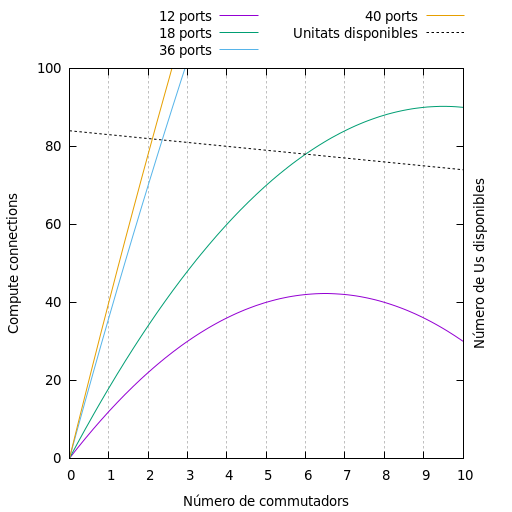
\includegraphics[width=0.8\linewidth]{img/connections.png}
    \caption{Connexions disponibles per a nodes de comput en funció del nombre de commutadors.}
    
    \label{fig:connections}
\end{figure}

